\documentclass{beamer}
\usepackage[orientation=portrait,size=a0,scale=1.4,debug]{beamerposter}
\mode<presentation>{\usetheme{ZH}}
\usepackage{chemformula}
\usepackage[utf8]{inputenc}
\usepackage[german, english]{babel} % required for rendering German special characters
\usepackage{siunitx} %pretty measurement unit rendering
\usepackage{hyperref} %enable hyperlink for urls
\usepackage{ragged2e}
\usepackage{color}
\usepackage{amsmath}
\usepackage{amssymb}
\usepackage{natbib}
\usepackage[skins,theorems]{tcolorbox}
\tcbset{highlight math style={enhanced,
  colframe=red,colback=white,arc=0pt,boxrule=1pt}}
% \usepackage{tikz}
% \newcommand\tikzmark[1]{%
%   \tikz[remember picture,overlay]\node(#1) {};%
% }
%
% \newcommand\Connect[3][]{%
% \tikz[remember picture,overlay]
%   \draw[->,red,>=latex,#1] (#2.north east) - ($ (#3.north west) + (-20pt,0) $ );%
% }
\usepackage{tikz}
\usetikzlibrary{positioning}


\usepackage{array,booktabs,tabularx}
\newcolumntype{Z}{>{\centering\arraybackslash}X} % centered tabularx columns

\title{\huge The Cosmic Abundance of Molecular Hydrogen}
\author{Thomas Fletcher, Supervisor: Dr.\,Amélie Saintonge}
\institute{Department of Physics and Astronomy, University College London}
\date{June 29, 2016}

\newlength{\columnheight}
\setlength{\columnheight}{105cm}

\begin{document}
\begin{frame}
\begin{columns}
	\begin{column}{.5\textwidth}
		\begin{beamercolorbox}[center,wd=\textwidth]{postercolumn}
			\begin{minipage}[T]{.95\textwidth}  % tweaks the width, makes a new \textwidth
				\parbox[t][\columnheight]{\textwidth}{ % must be some better way to set the the height, width and textwidth simultaneously
%%%%%%%%%%%%%%%%%%%%%%%%%%%%%%%%%%%%%%%%%%%%%%%%%%%%%%%%%%%%%%%%%%%%%%%%%%%%%%%%
					\begin{myblock}{\LARGE Introduction}
            The formation and evolution of galaxies is closely tied to the
            abundance of gas. Indeed, galaxy growth is regulated by the careful balance
            of its gas through inflows, outflows, star formation and the build
            up of its gas reservoir. It is therefore necessary to have a good
            understanding of the cosmic abundance of molecular gas
            $\Omega_{\text{H2}}$ throughout the history of the
            universe to understand galaxy growth and to constrain galaxy
            evolution models. \vspace{1ex}

            Previous research has derived $\Omega_{\text{H2}}$ using a biased sample of
            200 galaxies, most of which are irregular galaxies (spirals and
            mergers) \cite{keres2003co}. However,~$\approx~85~\%$ of the star
            formation budget of the Universe originates from normal
            main-sequence star forming galaxies. \vspace{1ex}

            COLD GASS is a survey that has charted the molecular gas content of
            local galaxies by measuring their CO(1-0) emission. Galaxies in
            the {COLD\,GASS} survey were selected based solely on their
            mass and redshift. Therefore, COLD GASS provides an unbiased and
            complete picture of molecular gas in local main-sequence
            star-forming galaxies. The purpose of this project is
            to use the COLD GASS sample to calculate a more representative
            estimate for $\mathrm{\Omega_{H2}}$.
					\end{myblock}\vfill
%%%%%%%%%%%%%%%%%%%%%%%%%%%%%%%%%%%%%%%%%%%%%%%%%%%%%%%%%%%%%%%%%%%%%%%%%%%%%%%%
					\begin{myblock}{\LARGE COLD GASS Data}

            \begin{itemize}
              \item The CO Luminosity $\mathrm{L_{CO}}$ is calculated from the
              integrated line flux $\mathrm{S_{CO}}$
              \item The conversion factor was calculated using the prescription
              given in \cite{genzel2012metallicity} for low mass, low metallicity
              galaxies whereas for high mass galaxies the galactic conversion
              factor was used.
              \item The molecular hydrogen mass function was calculated using
              just the detections and both the detections
              and the upper limits from the non-detections from the COLD GASS
              survey.
            \end{itemize}

						\begin{figure}[H]
						  \centering
						  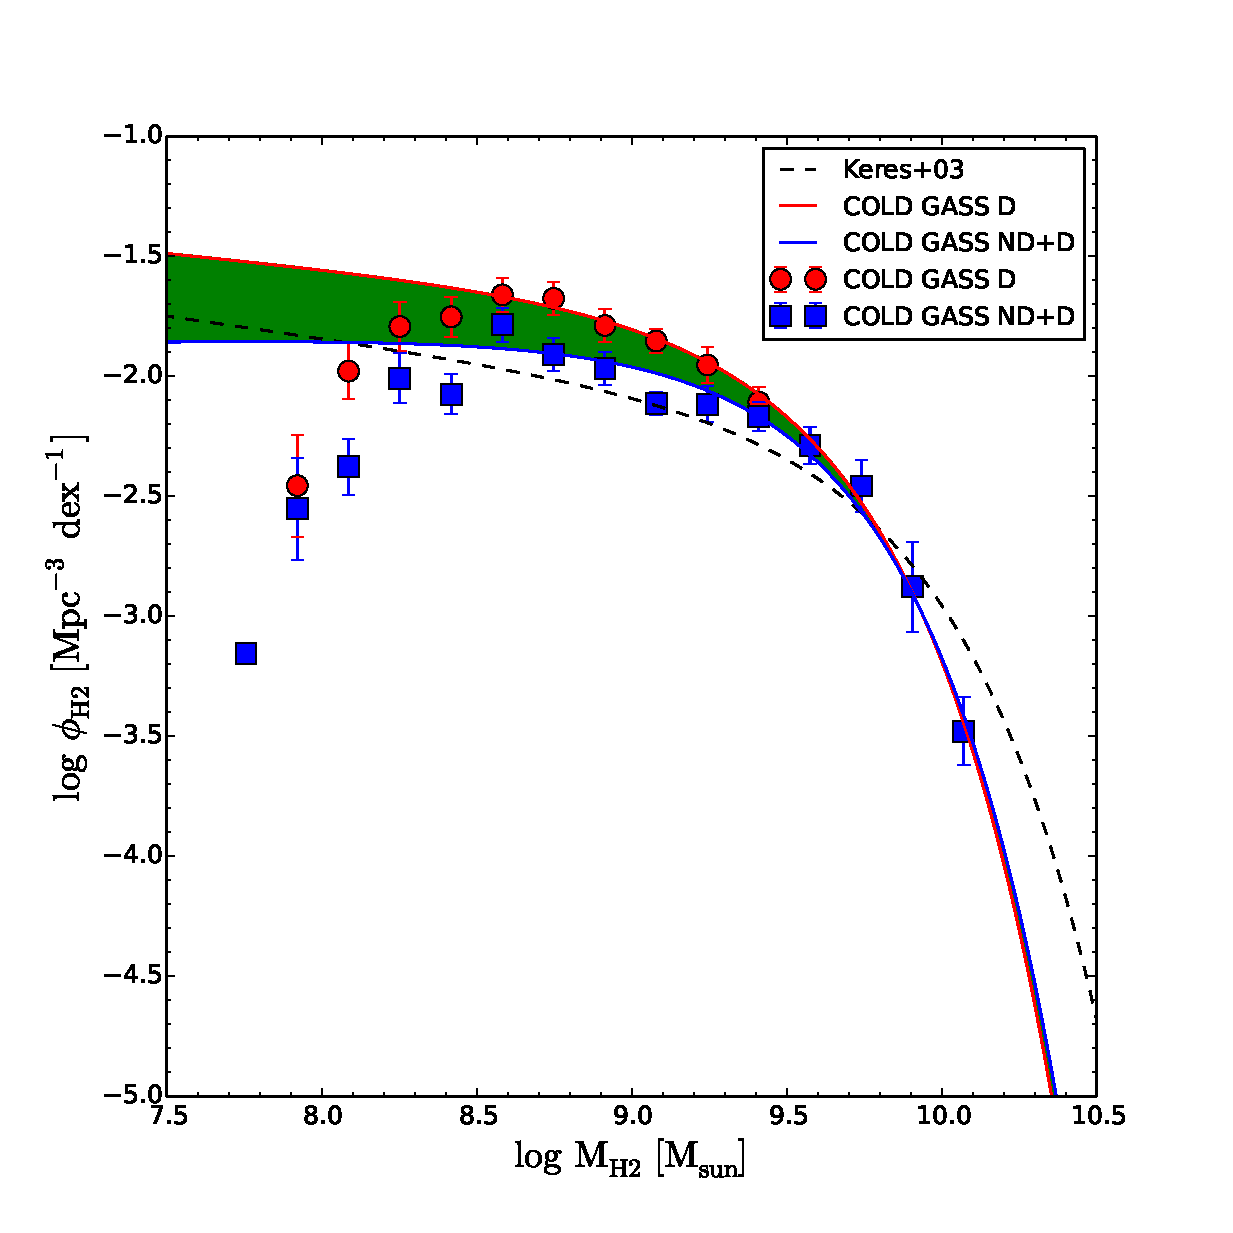
\includegraphics[width=\textwidth]{img/MH2poster.eps}
						  \caption{Molecular gas mass function ($\mathrm{M_{H2}}$).
							The blue squares represent the total number density of galaxies
              when only the detections from COLD GASS are used (D). The red circles
              show the number density when the upper limits from the non-detections
              are combined with the detections (ND+D). The dashed line is the best fit
              from \cite{keres2003co} and the blue and red solid lines show the
              best fit to the D and ND+D COLD GASS data respectively. The true
              answer lies somwehere within the green shaded region}
						  \label{fig:CG}
						\end{figure}
            In \cite{keres2003co} it was found that
            $\mathrm{\Omega_{H2} = 1.6 \pm 0.6 \times 10^{-4}}$
						\begin{equation}
							\tcbhighmath[drop fuzzy shadow]{\mathrm{\rho_{H2} = 2.7 \cdot 10^{7} ~ M_{\odot}~ Mpc^{-3}}}
						\end{equation}
					\end{myblock}\vfill
%%%%%%%%%%%%%%%%%%%%%%%%%%%%%%%%%%%%%%%%%%%%%%%%%%%%%%%%%%%%%%%%%%%%%%%%%%%%%%%%
\begin{myblock}{\LARGE Conclusions}
\end{myblock}\vfill
%%%%%%%%%%%%%%%%%%%%%%%%%%%%%%%%%%%%%%%%%%%%%%%%%%%%%%%%%%%%%%%%%%%%%%%%%%%%%%%%
		}\end{minipage}\end{beamercolorbox}
	\end{column}
%%%%%%%%%%%%%%%%%%%%%%%%%%%%%%%%%%%%%%%%%%%%%%%%%%%%%%%%%%%%%%%%%%%%%%%%%%%%%%%%
	\begin{column}{.5\textwidth}
		\begin{beamercolorbox}[center,wd=\textwidth]{postercolumn}
			\begin{minipage}[T]{.95\textwidth} % tweaks the width, makes a new \textwidth
				\parbox[t][\columnheight]{\textwidth}{ % must be some better way to set the the height, width and textwidth simultaneously
%%%%%%%%%%%%%%%%%%%%%%%%%%%%%%%%%%%%%%%%%%%%%%%%%%%%%%%%%%%%%%%%%%%%%%%%%%%%%%%%

%%%%%%%%%%%%%%%%%%%%%%%%%%%%%%%%%%%%%%%%%%%%%%%%%%%%%%%%%%%%%%%%%%%%%%%%%%%%%%%%
					\begin{myblock}{\LARGE Scaling Relations}
            To circumvent the inherent Malmquist bias in the COLD GASS data a
            second method that takes advantage of the tight scaling relations
            in the $\mathrm{M_{*}-SFR}$ \citep{saintonge2016SFRMstar} and
            $\mathrm{M_{H2}-SFR}$ planes is used.\vspace{1ex}

						\begin{itemize}
							\item \textbf{Step 1:} The double schechter fit (red and blue galaxies) for galaxy stellar mass function from the GAMA survey \citep{baldry2012galaxy} is used.
							\item \textbf{Step 2:} From this fit red and blue galaxy populations are constructed with a distribtuion across $\mathrm{M_{*}}$
							\item \textbf{Step 3:} Main sequence galaxies are assigned a $\mathrm{SFR}$ using the prescription in \cite{saintonge2016SFRMstar}. Red galaxies are given a lower SFR with some spread.
							\item \textbf{Step 4:} The tight scaling relation between $\mathrm{M_{H2}-SFR}$ is used to calculate the molecular hydrogen gas mass for each galaxy
							\item \textbf{Step 5:} The molecular hydrogen mass function is then plotted and  $\mathrm{\Omega_{H2}}$ is calculated.
						\end{itemize}
						% \begin{figure}
						% 	\begin{minipage}{0.4\textwidth}
						% 		\centering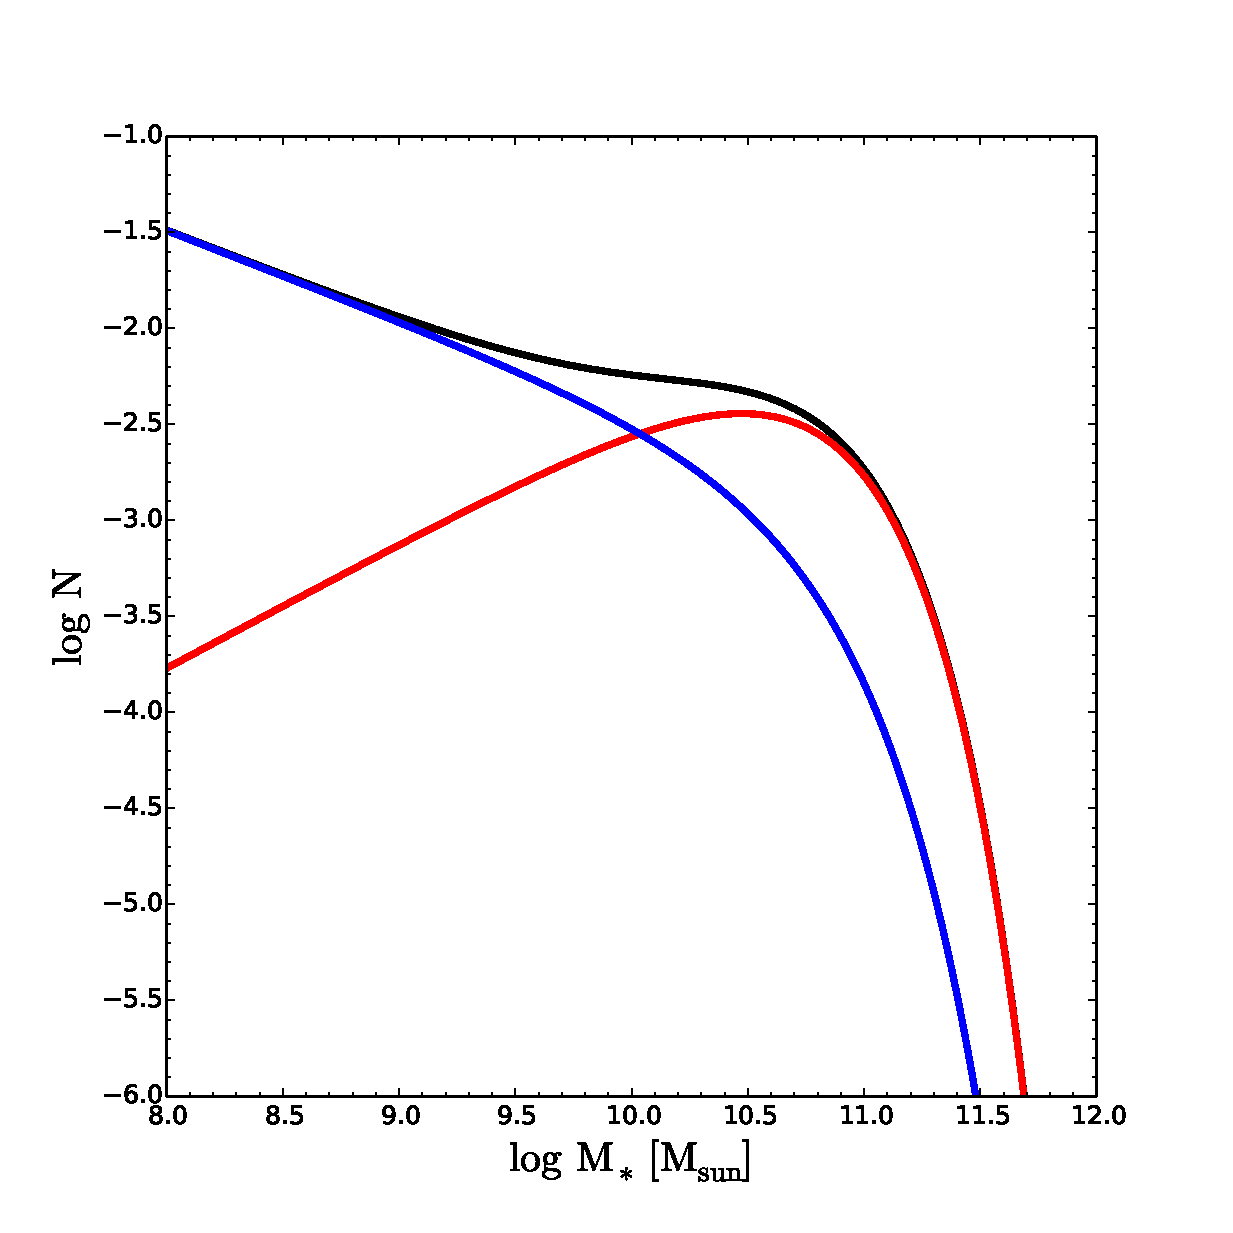
\includegraphics[width=\textwidth]{img/Baldry.eps}
						% 		\caption{\cite{baldry2012galaxy}}
						% 	\end{minipage}
						% 	\begin{minipage}{0.4\textwidth}
            %
						% 		\centering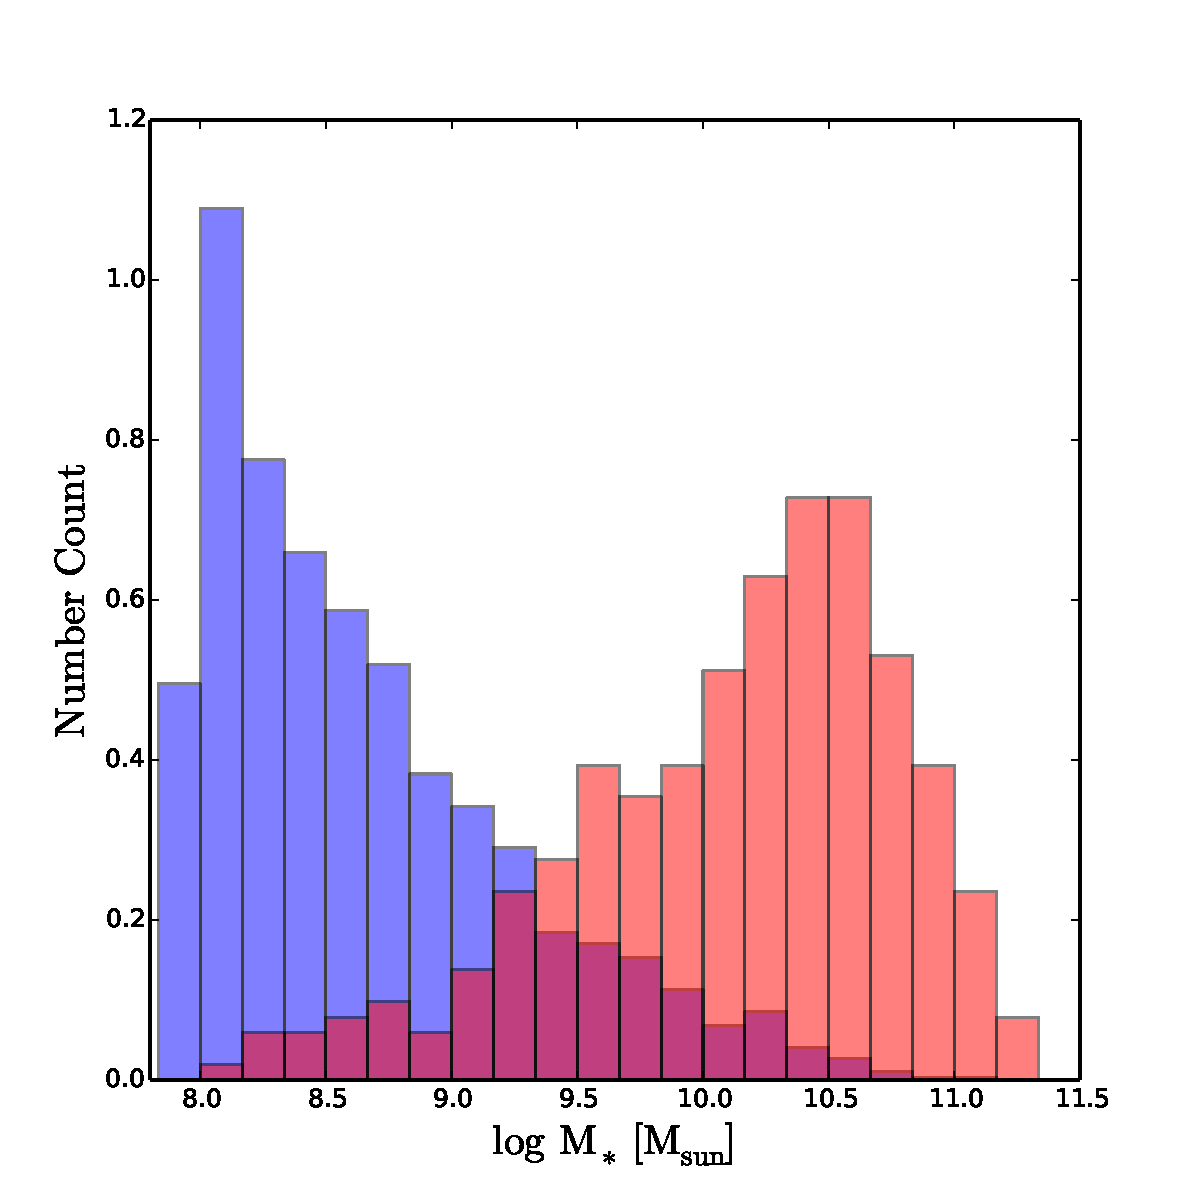
\includegraphics[width=\textwidth]{img/Hist.pdf}
						% 		\caption{}
						% 	\end{minipage}
						% \end{figure}
            %
            % % \begin{tikzpicture}[remember picture,overlay]
            % %   \Connect{start1}{end1}
            % % \end{tikzpicture}
            %
						% \begin{figure}
						% 	\begin{minipage}{0.4\textwidth}
						% 		\centering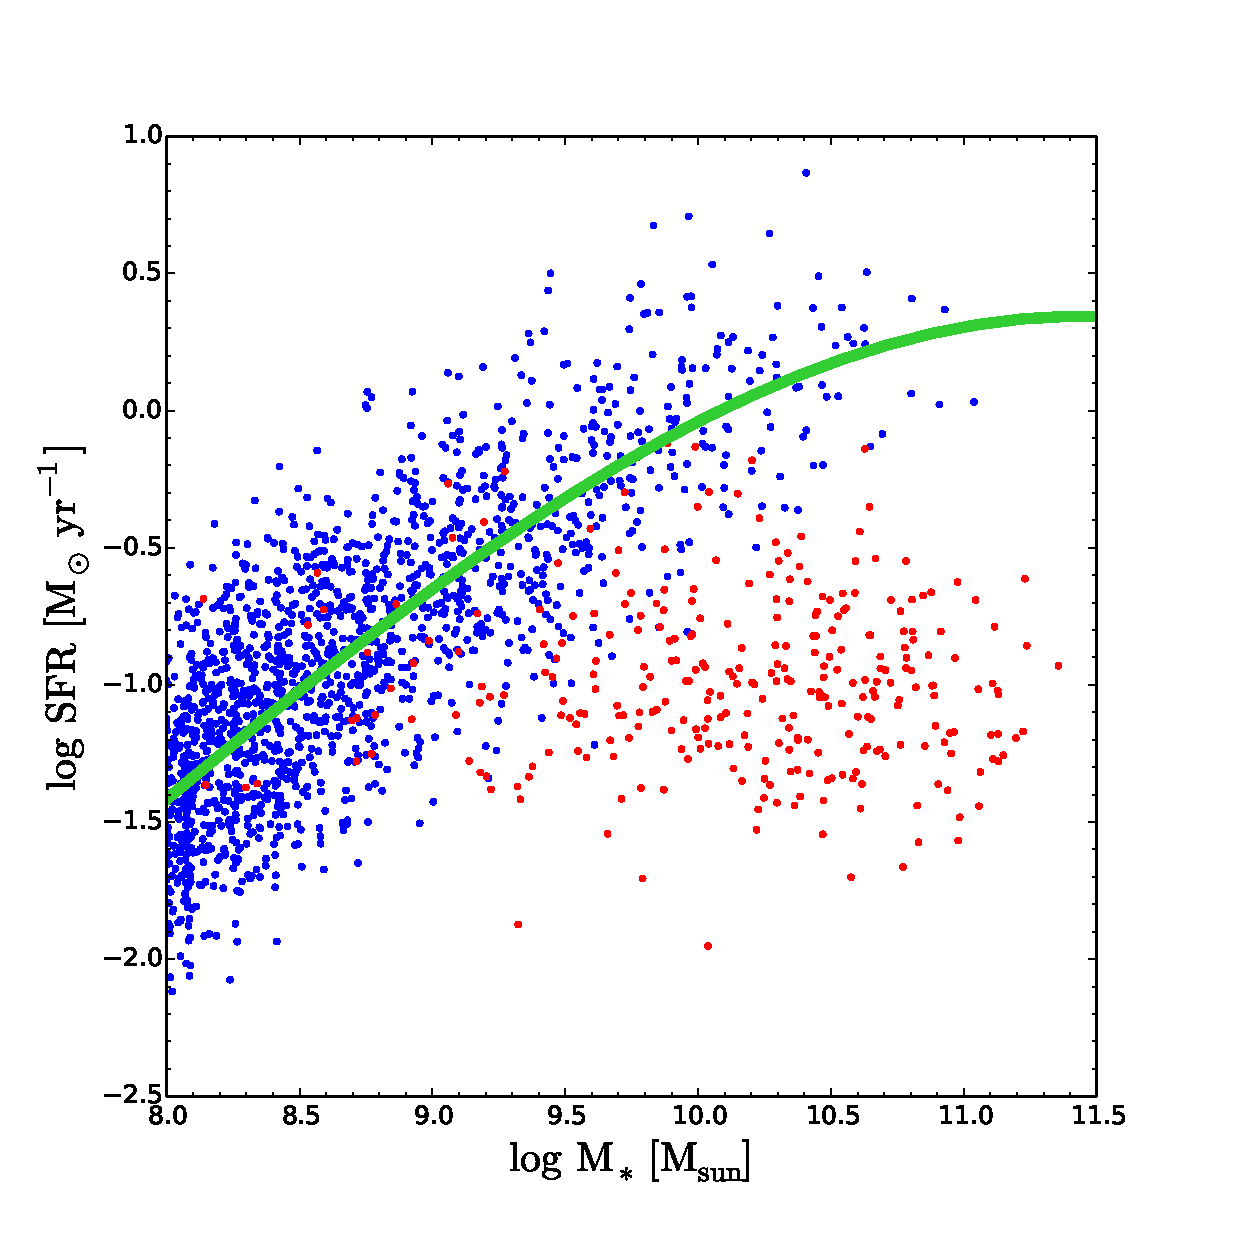
\includegraphics[width=\textwidth]{img/MSFR.eps}
						% 		\caption{\cite{saintonge2016SFRMstar}}
						% 	\end{minipage}
						% 	\begin{minipage}{0.4\textwidth}
						% 		\centering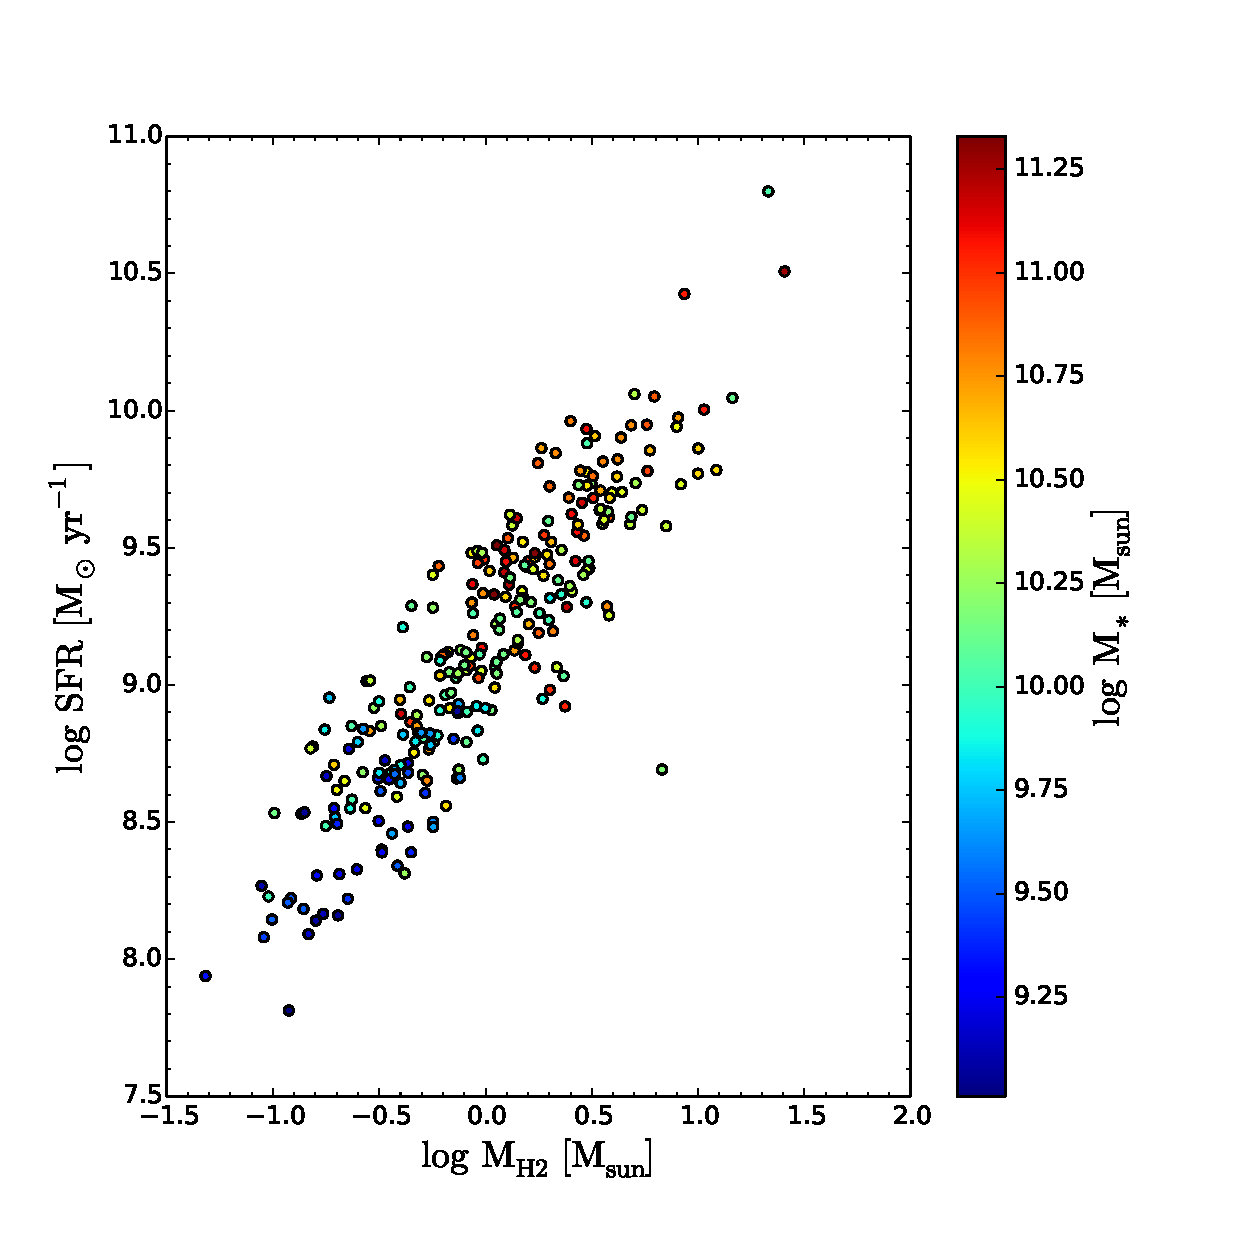
\includegraphics[width=\textwidth]{img/scalrelns.eps}
						% 		\caption{}
						% 	\end{minipage}
						% \end{figure}
            %
            % \begin{figure}[H]
						%   \centering
						%   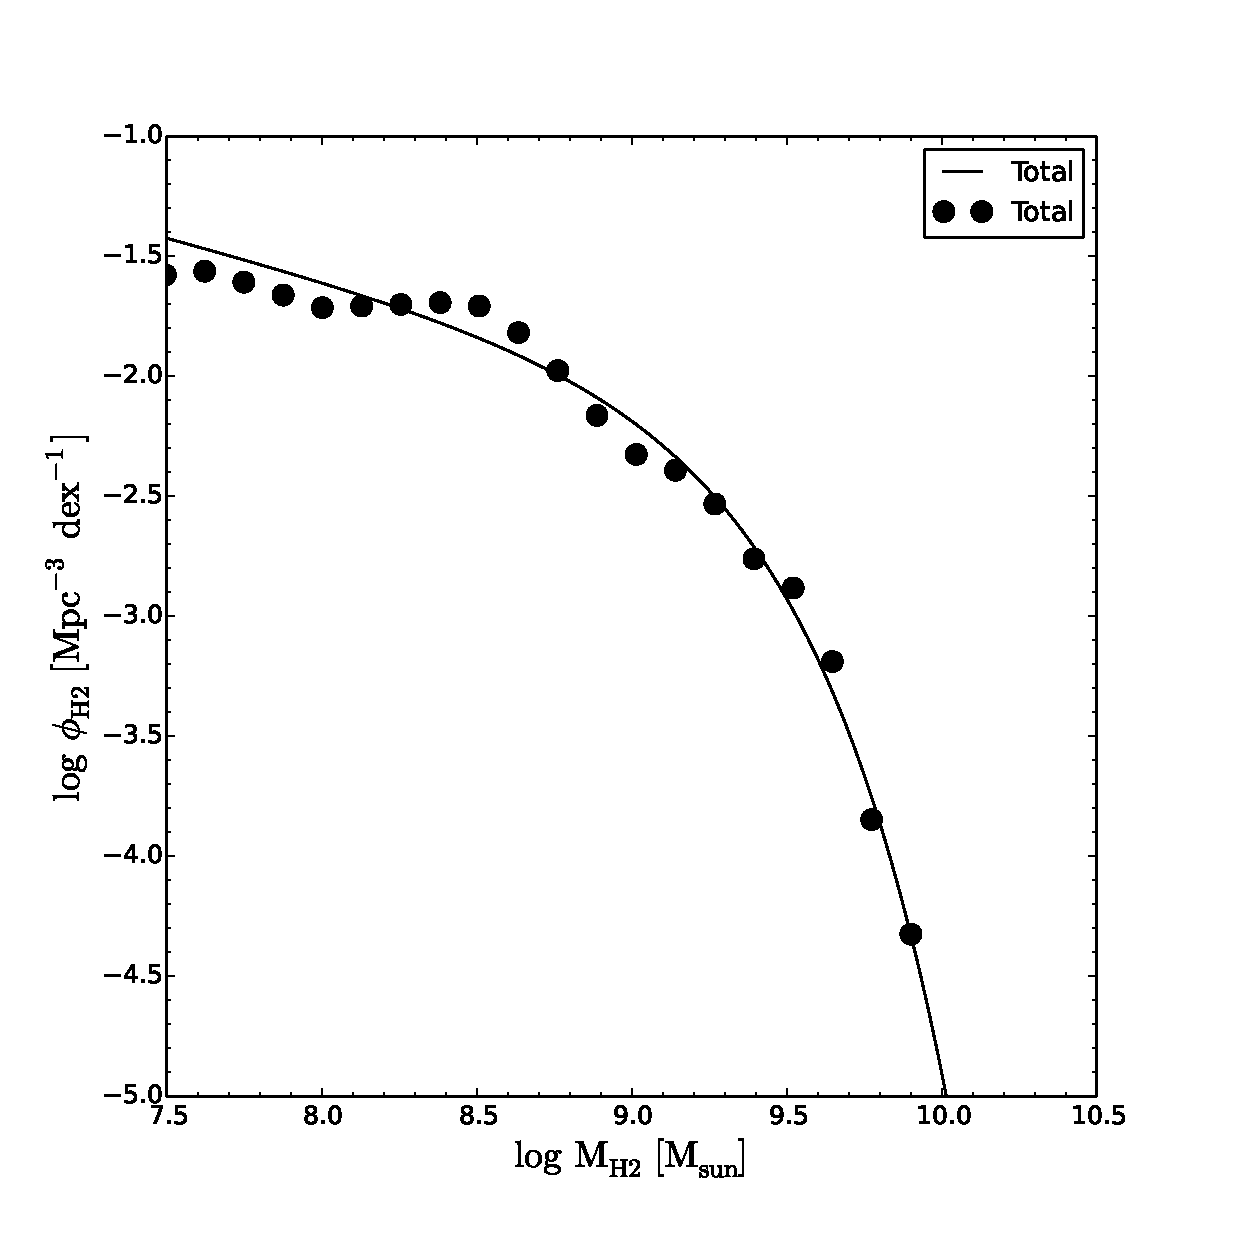
\includegraphics[width=0.5\textwidth]{img/MH2scal.eps}
						%   \caption{}
						%   \label{fig:scal}
						% \end{figure}
            \begin{figure}
              \begin{tikzpicture}
              \node (baldry) [left = 1cm]{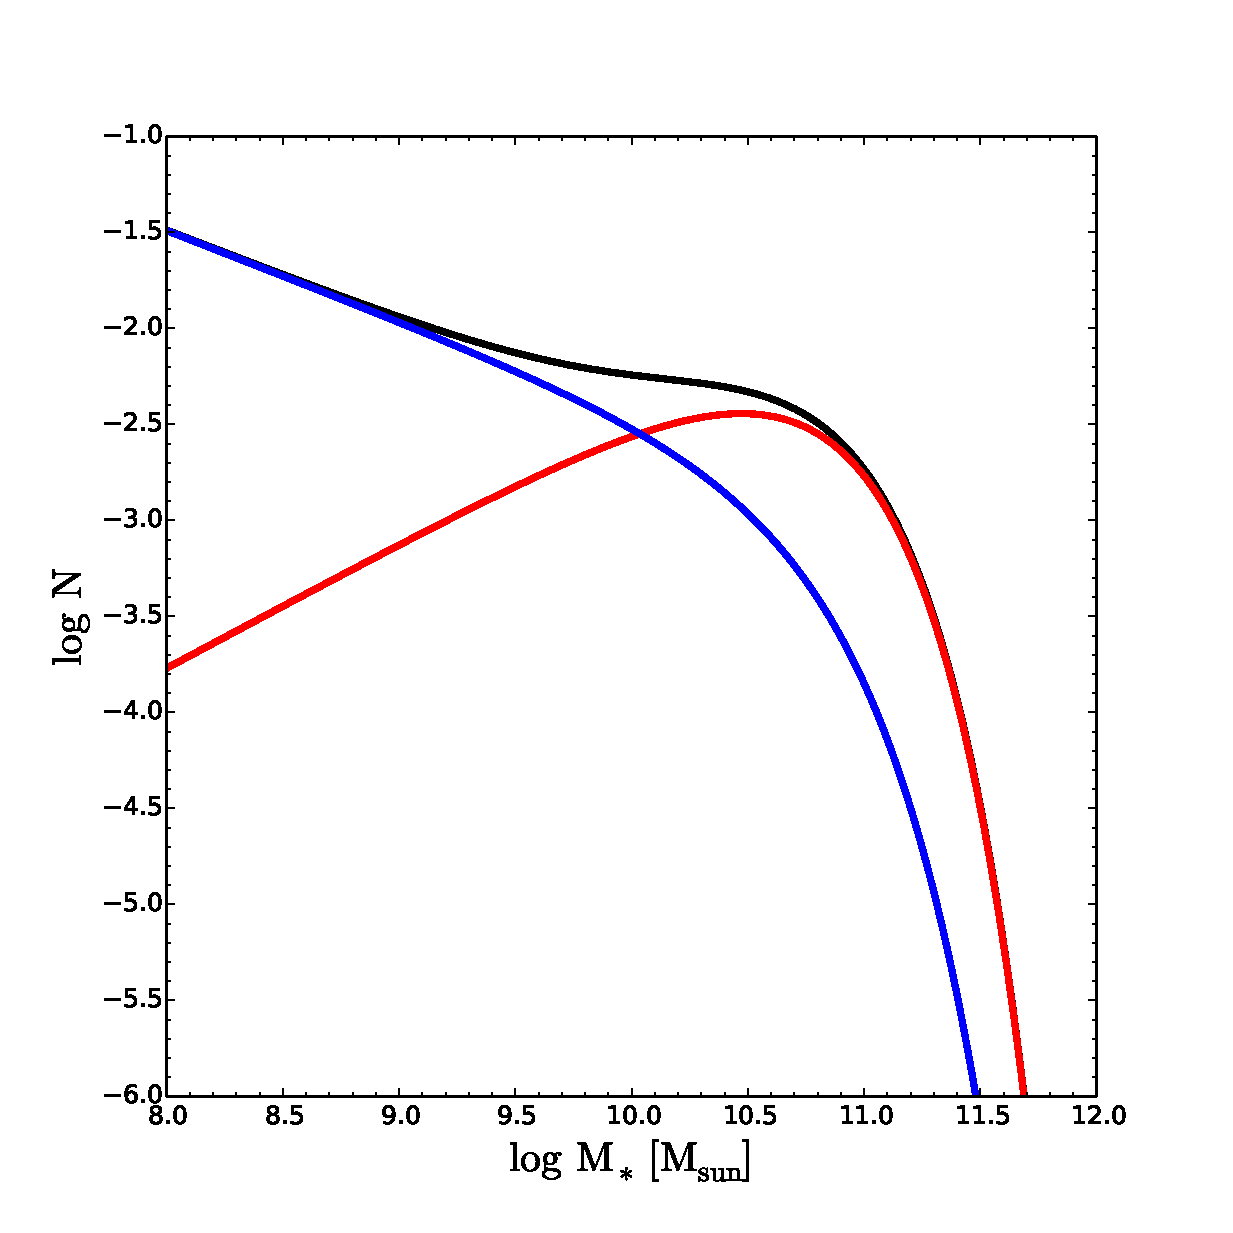
\includegraphics[width=0.4\textwidth]{img/Baldry.eps}};
              \node (histo) [right=of baldry 2.5cm] {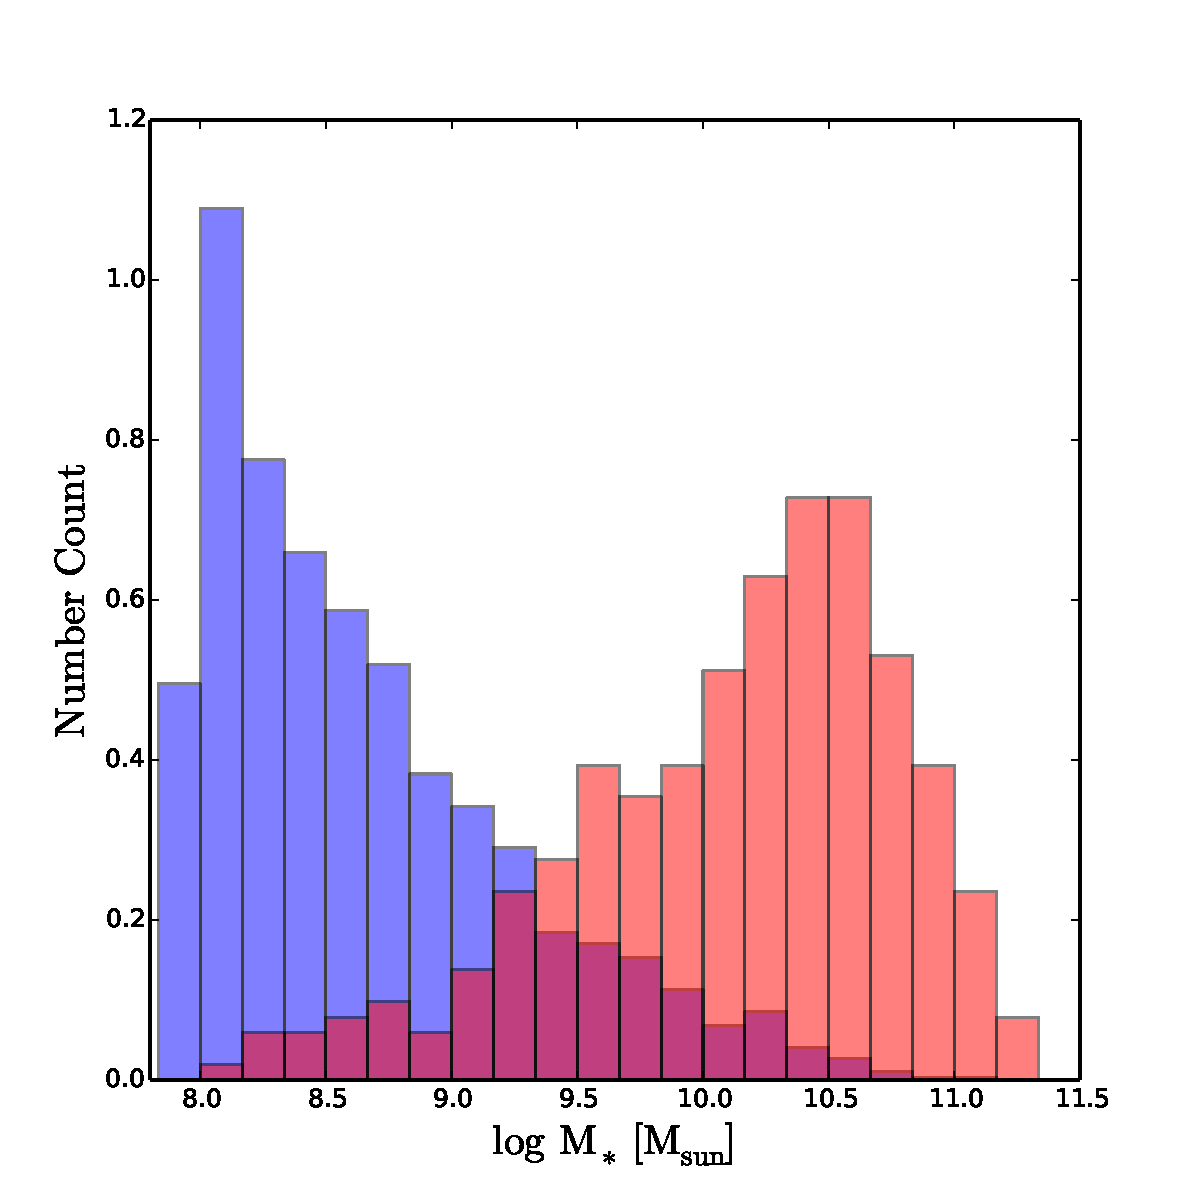
\includegraphics[width=0.4\textwidth]{img/Hist.pdf}};
              \node (MSFR) [below=of baldry] {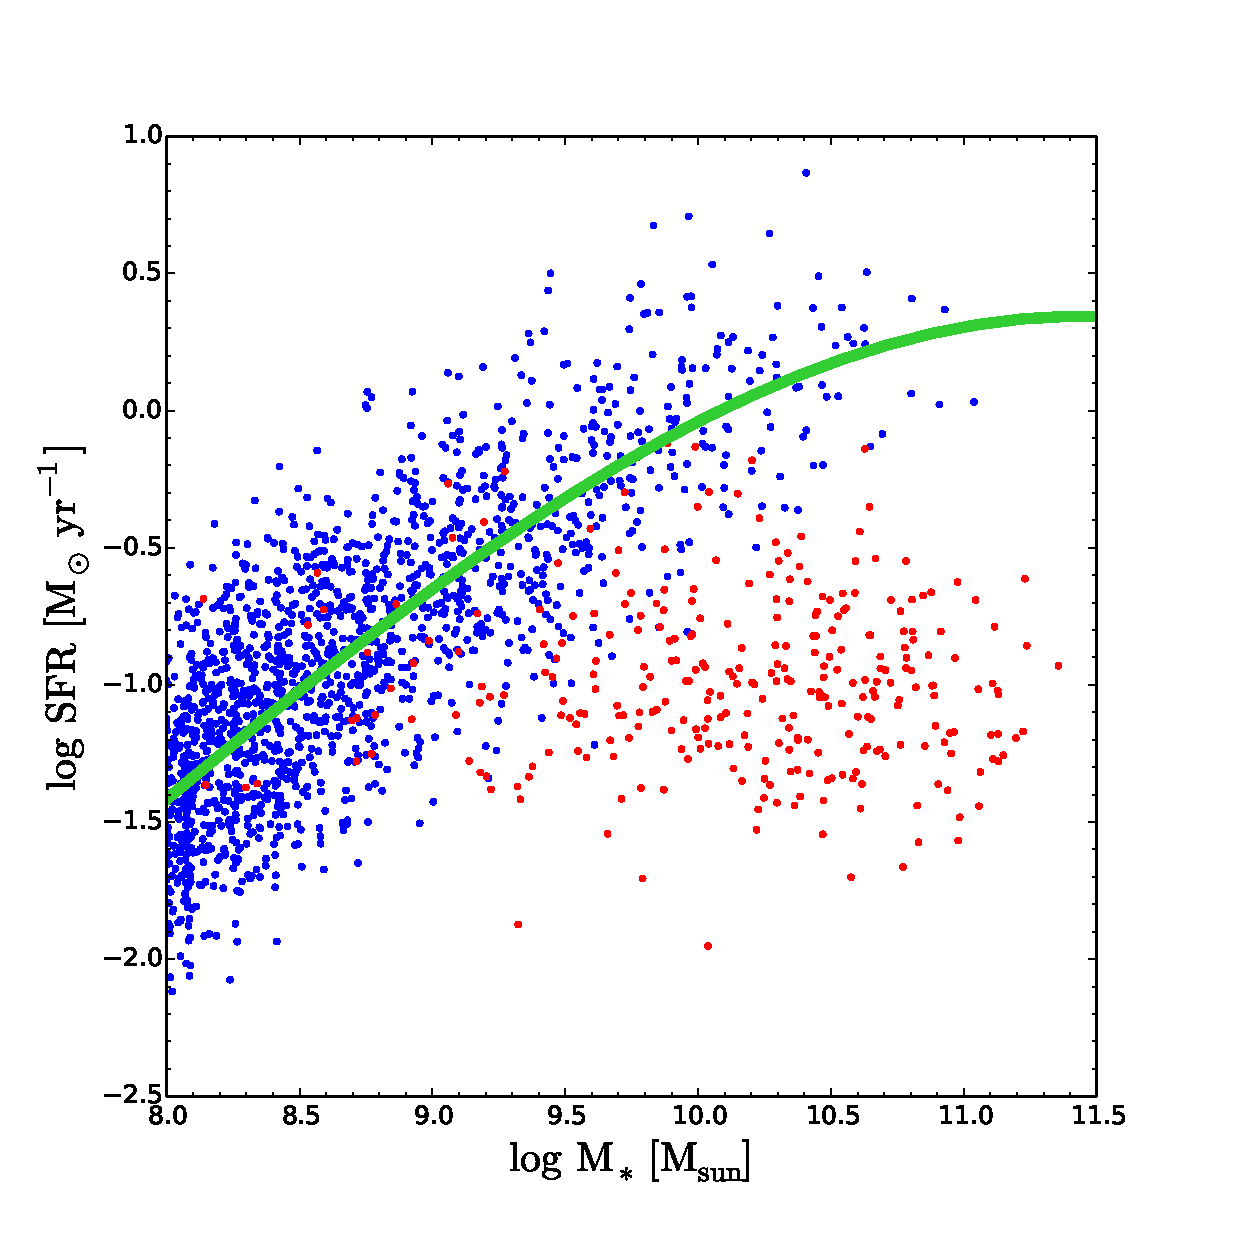
\includegraphics[width=0.4\textwidth]{img/MSFR.eps}};
              \node (gio) [below=of histo] {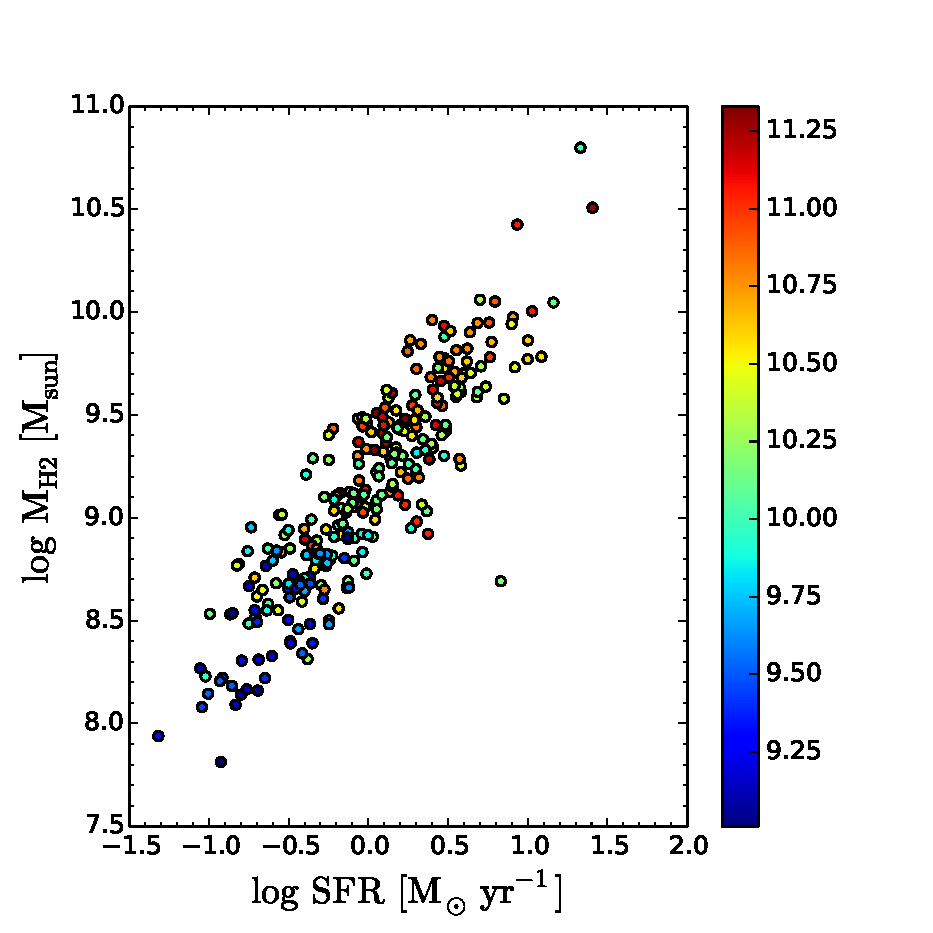
\includegraphics[width=0.4\textwidth]{img/scalrelns2.eps}};
              \node (sch) [below=of MSFR] {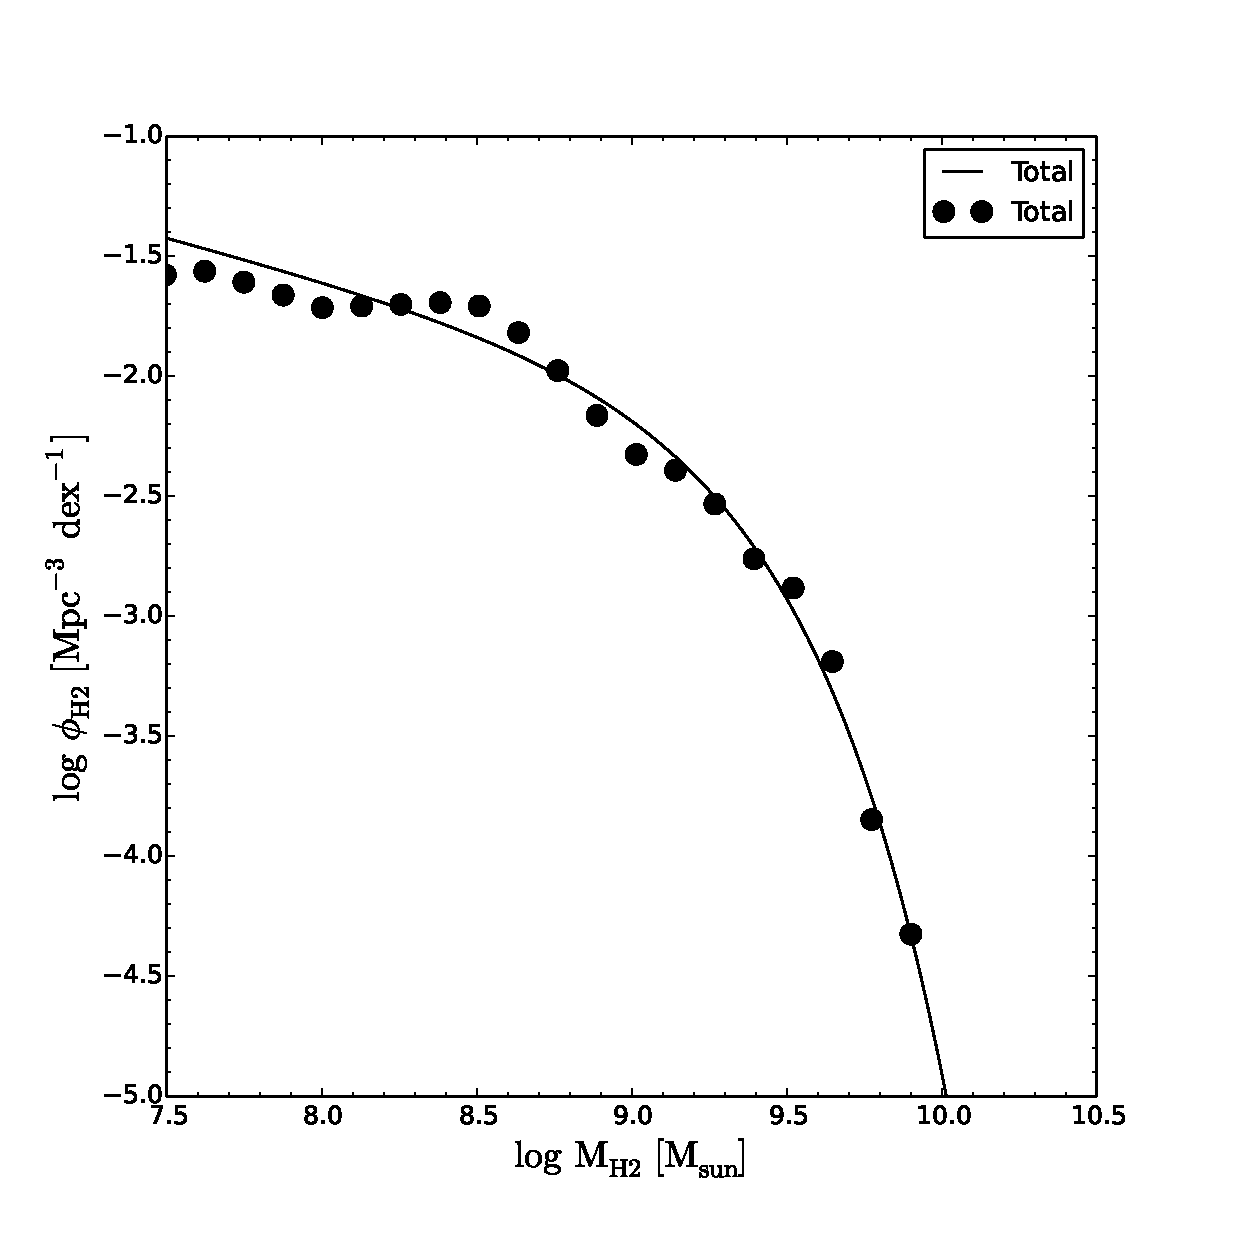
\includegraphics[width=0.4\textwidth]{img/MH2scal.eps}};
              \node (eqn) [right=of sch] {\begin{equation}\tcbhighmath[drop fuzzy shadow]{\mathrm{\rho_{H2} = ? \cdot 10^{7} ~ M_{\odot}~ Mpc^{-3}}}\end{equation}};
              \draw [line width = 3mm,red, ->] (baldry) to (histo);
              \draw [line width = 3mm,,red,->] (histo) to (MSFR);
              \draw [line width = 3mm,,red,->] (MSFR) to (gio);
              \draw [line width = 3mm,,red,->] (gio) to (sch);
              \end{tikzpicture}
            \end{figure}
					\end{myblock}\vfill
%%%%%%%%%%%%%%%%%%%%%%%%%%%%%%%%%%%%%%%%%%%%%%%%%%%%%%%%%%%%%%%%%%%%%%%%%%%%%%%%
					\begin{myblock}{\LARGE References}
						\footnotesize
						\bibliographystyle{agsm}
						\bibliography{./bib}
					\end{myblock}\vfill
%%%%%%%%%%%%%%%%%%%%%%%%%%%%%%%%%%%%%%%%%%%%%%%%%%%%%%%%%%%%%%%%%%%%%%%%%%%%%%%%
		}\end{minipage}\end{beamercolorbox}
	\end{column}
\end{columns}
\end{frame}
\end{document}
